\newpage
\subsection{Log Messages}
\subsubsection{Ausgangslage}
Eine VPN Tunnel wurde mit Hilfe des strongMan korrekt konfiguriert und steht nun bereit für den Auf- und Abbau.
Der Tunnel wird gestartet, dies lösst auf der Client Seite einen Asynchronen Request aus, der auf dem Backend die Daten des konfigurierten Tunnels aus der Datenbank liest und in eine passende Form für die VICI Schnittstelle aufbereiten und übergibt. Die geladene Verbindung wird nun gestartet, was zur Folge hat, dass blockierend ein Generator zurück gegeben wird. Welcher jede neue Nachricht in die Datenbank loggt.

\subsubsection{Problematik}
Die Log Nachrichten werden durch einen Thread, dessen Laufzeit nicht bekannt ist, mit Hilfe des Generators in die Datenbank geschrieben. Der Thread terminiert, wenn ein Tunnel aufgebaut wurde oder falls dies nicht möglich war erst nach mehreren Retry versuchen. Während dieser Zeit werden diverse Logs gespeichert, die dem Benutzer möglichst in Echtzeit angezeigt werden sollten. 

\subsubsection{Lösungsansatz}
Das laden der Connection Overview Seite lösst einen Long Polling Request aus, der alle zuest alle Logs die älter als 5 Minuten sind aus der Datenbank löscht und die restlichen dem Frontend zurück gibt. Die führt dazu , dass ein neuer Long Polling Request gestartet wird, welcher den neusten Log als Parameter mit gibt und nun nur noch neuere Meldungen übermittelt werden. Dies wird wiederholt, bis die Connection Overview Seite verlassen wird.
\medskip
\begin{figure}[H]
\centering
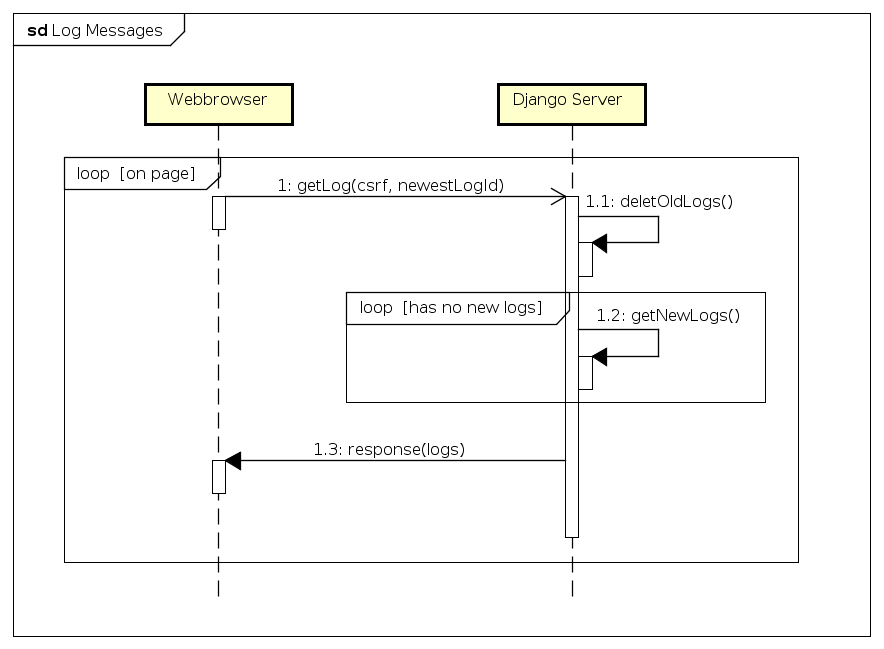
\includegraphics[width=400pt]{images/log_messages_seq.png}
\caption[Log Messages Sequenzdiagramm]{Log Messages Sequenzdiagramm}
\end{figure}